\documentclass[12pt, a4paper]{article}

% ─── Packages ───────────────────────────────────────────────────────────────
\usepackage[T1]{fontenc}
\usepackage[utf8]{inputenc}
\usepackage[english]{babel}
\usepackage{geometry}
\usepackage{graphicx}
\usepackage{xcolor}
\usepackage{titlesec}
\usepackage{titletoc}
\usepackage{fancyhdr}
\usepackage{parskip}
\usepackage{hyperref}
\usepackage[protrusion=true,expansion=false]{microtype}
\usepackage{enumitem}
\usepackage{booktabs}
\usepackage{array}
\usepackage{caption}
\usepackage{tikz}
\usetikzlibrary{shapes.geometric, arrows.meta, positioning, fit, backgrounds}
\usepackage{amsmath}
\usepackage{amssymb}
\usepackage{setspace}
\usepackage{tocloft}
\usepackage{float}

% ─── Page geometry ────────────────────────────────────────────────────────────
\geometry{
  a4paper,
  top=2.5cm, bottom=2.5cm,
  left=2.5cm, right=2.5cm,
  headheight=15pt
}

% ─── IMT Atlantique colours ───────────────────────────────────────────────────
\definecolor{imtblue}{RGB}{0, 83, 120}
\definecolor{imtteal}{RGB}{0, 156, 166}
\definecolor{imtgreen}{RGB}{134, 188, 121}
\definecolor{imtgray}{RGB}{100, 100, 100}

% ─── Section heading styles ──────────────────────────────────────────────────
\titleformat{\section}
  {\large\bfseries\color{imtblue}}
  {\thesection.}{0.5em}{}[\vspace{-4pt}\rule{\linewidth}{0.4pt}]

\titleformat{\subsection}
  {\normalsize\bfseries\color{imtteal}}
  {\thesubsection.}{0.5em}{}

\titleformat{\subsubsection}
  {\normalsize\itshape\color{imtgray}}
  {\thesubsubsection.}{0.5em}{}

\titlespacing{\section}{0pt}{14pt}{6pt}
\titlespacing{\subsection}{0pt}{10pt}{4pt}

% ─── Table of contents styling ────────────────────────────────────────────────
\renewcommand{\cftsecfont}{\bfseries\color{imtblue}}
\renewcommand{\cftsubsecfont}{\color{imtteal}}
\renewcommand{\cftsecpagefont}{\bfseries}
\renewcommand{\cfttoctitlefont}{\Large\bfseries\color{imtblue}}
\renewcommand{\cftdot}{.}
\setlength{\cftbeforesecskip}{4pt}

% ─── Headers and footers ─────────────────────────────────────────────────────
\pagestyle{fancy}
\fancyhf{}
\fancyhead[L]{\small\color{imtgray}\leftmark}
\fancyhead[R]{\small\color{imtgray}\thepage}
\fancyfoot[C]{\small\color{imtgray}\rule{0.4\linewidth}{0.3pt}}
\renewcommand{\headrulewidth}{0pt}

% ─── Hyperref ────────────────────────────────────────────────────────────────
\hypersetup{
  colorlinks=true,
  linkcolor=imtblue,
  urlcolor=imtteal,
  citecolor=imtblue,
}

% ─── Caption style ───────────────────────────────────────────────────────────
\captionsetup{
  font=small,
  labelfont={bf,color=imtteal},
  textfont={it,color=imtgray},
  labelsep=period,
}

% ─── TikZ styles ─────────────────────────────────────────────────────────────
\tikzset{
  agent/.style={
    rectangle, rounded corners=4pt,
    draw=imtblue, fill=imtblue!8,
    text width=2.8cm, align=center,
    minimum height=1cm, font=\small\bfseries
  },
  smallbox/.style={
    rectangle, rounded corners=3pt,
    draw=imtteal, fill=imtteal!10,
    text width=2.2cm, align=center,
    minimum height=0.8cm, font=\footnotesize
  },
  arr/.style={-Stealth, thick, color=imtblue},
  darr/.style={-Stealth, thick, color=imtteal, dashed},
  placeholder/.style={
    draw=imtgray, dashed, line width=0.8pt,
    fill=gray!6, rounded corners=2pt
  },
}

% ─── Image placeholder helper ────────────────────────────────────────────────
% Usage: \imgplaceholder{width}{height}{caption text}{label}
\newcommand{\imgplaceholder}[4]{%
  \begin{figure}[H]
  \centering
  \begin{tikzpicture}
    \node[placeholder, minimum width=#1, minimum height=#2] (box) {};
    \node[color=imtgray, font=\itshape\small] at (box.center)
      {[Insert screenshot here]};
  \end{tikzpicture}
  \caption{#3}
  \label{#4}
  \end{figure}
}

% ════════════════════════════════════════════════════════════════════════════
\begin{document}

% ─── Title Page ──────────────────────────────────────────────────────────────
\begin{titlepage}
\thispagestyle{empty}

\begin{flushright}

\begin{tikzpicture}
  \fill[imtblue]  (0,0) -- (4,0) -- (4,4) -- cycle;
  \fill[imtgreen] (4,4) -- (4,2) -- (2,4) -- cycle;
  \fill[imtteal]  (4,0) -- (4,2) -- (2.5,0) -- cycle;
\end{tikzpicture}
\end{flushright}

\vspace{2.5cm}

{\color{imtblue}\LARGE\bfseries
MOOC Assistant --- Third Semester Report\\[8pt]
}
\vspace{2cm}

{\normalsize\color{imtgray}
Prepared by:\\[4pt]
\textbf{Tarun VENKATESH}
}

\vspace{1.2cm}

{\normalsize\color{imtgray}
Supervisors:\\[4pt]
Laurent TOUTAIN\\
Baptiste GAULTIER
}

\vfill


\begin{tikzpicture}
  \fill[imtblue]  (0,0)   -- (0.6,0) -- (0,0.6) -- cycle;
  \fill[imtteal]  (0.7,0) -- (1.3,0) -- (0.7,0.6) -- cycle;
  \fill[imtgreen] (1.4,0) -- (2.0,0) -- (1.4,0.6) -- cycle;
\end{tikzpicture}\\[2pt]
{\small\bfseries\color{imtblue} IMT Atlantique}\\
{\small\color{imtgray} Bretagne-Pays de la Loire\\École Mines-Télécom}

\vspace{0.5cm}
{\small\color{imtgray} Academic Year 2025--2026}

\end{titlepage}

% ─── Table of Contents ────────────────────────────────────────────────────────
\tableofcontents
\newpage

% ════════════════════════════════════════════════════════════════════════════
\section{Introduction}
\markboth{1. Introduction}{}

The MOOC Assistant project addresses a persistent challenge in large-scale online education: discussion forums accumulate student questions far faster than instructors can respond manually. In high-enrolment courses on the FUN-MOOC platform , individual instructors may face hundreds of unanswered posts spanning technical, conceptual, and administrative questions. The objective of this project is to build a multi-agent system that can automatically extract forum posts, generate course-grounded responses where appropriate, validate answer quality, and route uncertain or complex cases to human review .

The system is deliberately designed not as a single chatbot, but as a pipeline of specialised agents that collaborate to produce safer and more pedagogically reliable results. Each agent holds a distinct responsibility in the workflow, and their combined output is surfaced through a Streamlit dashboard that separates high-confidence automated responses from cases requiring instructor attention.

\subsection{Recap}

The establishment of the extraction and navigation foundation of the system. Using the Model Context Protocol (MCP) and Playwright browser automation, the system was built to log into the FUN-MOOC platform, navigate forum topic listing pages across multiple paginated views, and extract individual forum posts. Each post was parsed from the page's accessibility tree into a structured record containing the author username, post date, and post content.

The extractor agent successfully handled multi-page topics by detecting pagination links, navigating each page sequentially, and aggregating posts from all pages into a unified structure.
By the end of the first semester, the system could reliably log in, discover forum topics, navigate paginated threads, and produce structured post data with some AI generated responses. No Retrieval Augmented Generation or validation logic had been implemented at that stage.

\subsection{Current Objectives}

The focus was on expanding the pipeline beyond raw extraction and into intelligent response generation, quality control, and dashboard presentation \cite{kasneci2023chatgpt}. The specific objectives were: implementing Retrieval-Augmented Generation (RAG) to ground responses in real course material \cite{lewis2020rag}; modifying the solution agent that generates pedagogically appropriate responses in French; developing a validation agent that checks response quality before publication; implementing human-in-the-loop routing for uncertain cases \cite{gaultier2024mcp}; and redesigning the Streamlit dashboard to reflect the full pipeline state clearly.

% ════════════════════════════════════════════════════════════════════════════
\section{Implementations}
\markboth{2. Implementations}{}

The following components were designed, implemented, and integrated during the third semester of the project.

\begin{itemize}[leftmargin=1.5em, itemsep=4pt]

  \item \textbf{Semantic RAG pipeline.} A course ingestion script was written to parse HTML lesson files and XML exercise files from the edX course export into plain text chunks. A multilingual sentence embedding model \cite{reimers2020multilingual} was used to build a semantic vector index. A retriever module converts student questions into query embeddings and retrieves the most relevant course chunks at inference time using cosine similarity.

  \item \textbf{Forum post indexing.} After each extraction run, answered forum posts and their AI responses are appended to the RAG index. This incrementally enriches the knowledge base with real student questions over time.

  \item \textbf{Intent-aware post filtering.} The solution agent includes a multi-stage filtering layer that classifies each post before attempting generation. Posts from instructors are skipped entirely. Posts that are pure greetings, administrative questions, or complaint messages are routed to the professor review queue. Only posts that contain genuine technical or conceptual questions are forwarded for RAG-augmented answer generation.

  \item \textbf{RAG-augmented solution agent.} For qualifying posts, the agent retrieves relevant course context and injects it into a structured prompt sent to an LLM (Llama 3.1 via the Groq API). The prompt constrains the model to answer only from the retrieved context and instructs it to emit a special skip token if the context is insufficient.

  \item \textbf{Validation agent.} A two-stage validation pipeline evaluates every draft response before it appears in the dashboard. The first stage applies rule-based checks to catch obvious failures. The second stage uses a stronger LLM to score the response on relevance, grounding, and clarity, and to optionally rewrite it.

  \item \textbf{Human-in-the-loop (HITL) \cite{gaultier2024mcp}.} Posts that are ambiguous, administrative, low-relevance, or flagged by the validator are routed to a Professor Review queue. The dashboard shows the student post, the draft response and the validation scores so that the instructor has sufficient context to judge and optionally publish the answer.

  \item \textbf{Streamlit dashboard redesign.} The dashboard was restructured into three mutually exclusive views: \textit{Conversations and Responses} (automated answers), \textit{Professor Review} (flagged cases), and \textit{Others} (ignored posts). Sidebar counters provide an accurate breakdown of the pipeline state, and the count mismatch bug from the prototype was resolved by enforcing exclusive category assignment.

\end{itemize}

% ── Figure 2: Dashboard overview ─────────────────────────────────────────────
\begin{figure}[H]
\centering
\includegraphics[width=\linewidth]{dashboard_overview.png}
\caption{Overall dashboard layout showing the three-tab structure: Conversations \& Responses,
Professor Review, and Others, along with the sidebar counters displaying pipeline statistics.fig:dashboard
overview.}
\label{fig:dashboard-overview}
\end{figure}

% ════════════════════════════════════════════════════════════════════════════
\section{System Architecture}
\markboth{3. System Architecture}{}

\subsection{Architecture Overview}

The final architecture is organized into four specialized agents coordinated by an orchestrator, with a Streamlit dashboard providing the human interface. The agents communicate sequentially: the orchestrator directs the extractor, the extractor feeds the solution agent, the solution agent feeds the validator, and the validator's output determines whether a post enters the automated response track or the professor review track.

\begin{figure}[H]
\centering
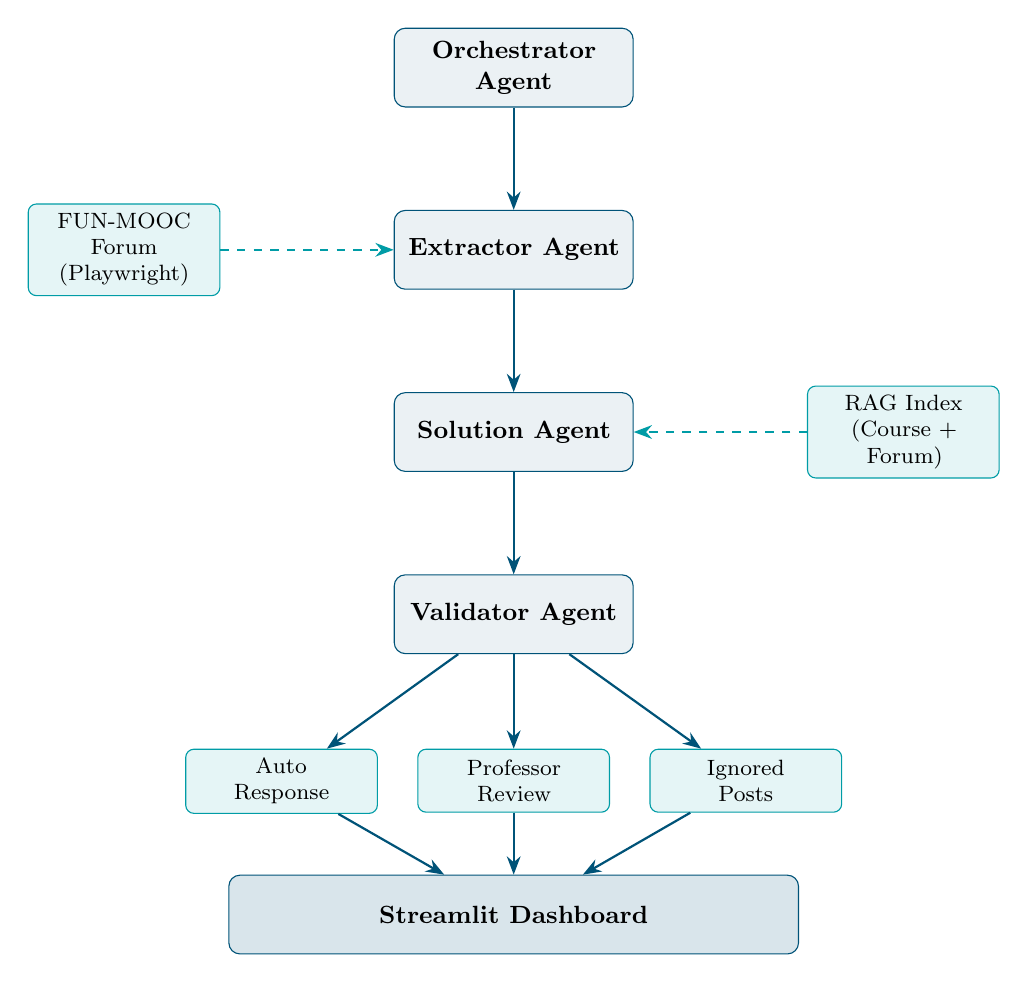
\begin{tikzpicture}[node distance=1.3cm and 1.6cm]

  % Nodes
  \node[agent] (orch)  {Orchestrator Agent};
  \node[agent, below=of orch] (ext)    {Extractor Agent};
  \node[agent, below=of ext]  (sol)    {Solution Agent};
  \node[agent, below=of sol]  (val)    {Validator Agent};

  % RAG box
  \node[smallbox, right=2.2cm of sol] (rag) {RAG Index\\ (Course +\\ Forum)};

  % Dashboard outputs
  \node[smallbox, below left=1.2cm and 0.2cm of val]  (auto) {Auto\\ Response};
  \node[smallbox, below=1.2cm of val]                 (hitl) {Professor\\ Review};
  \node[smallbox, below right=1.2cm and 0.2cm of val] (ign)  {Ignored\\ Posts};

  % Dashboard
  \node[agent, below=2.8cm of val, fill=imtblue!15, draw=imtblue,
        text width=7cm] (dash) {Streamlit Dashboard};

  % FUN-MOOC
  \node[smallbox, left=2.2cm of ext] (forum) {FUN-MOOC\\ Forum\\ (Playwright)};

  % Arrows
  \draw[arr] (orch) -- (ext);
  \draw[arr] (ext)  -- (sol);
  \draw[arr] (sol)  -- (val);
  \draw[darr] (rag) -- (sol);
  \draw[darr] (forum) -- (ext);

  \draw[arr] (val) -- (auto);
  \draw[arr] (val) -- (hitl);
  \draw[arr] (val) -- (ign);

  \draw[arr] (auto) -- (dash);
  \draw[arr] (hitl) -- (dash);
  \draw[arr] (ign)  -- (dash);

\end{tikzpicture}
\caption{Full system architecture of the MOOC Assistant pipeline.}
\label{fig:arch}
\end{figure}

\subsection{Component Descriptions}

\textbf{Orchestrator Agent.} The orchestrator is responsible for driving the entire pipeline. It calls the extractor to collect forum posts from a configurable set of topic pages, then iterates over each extracted post and passes it through the solution and validator agents. After each topic is processed, it also calls the RAG indexer to add newly answered posts to the knowledge base. The orchestrator aggregates the final counts and topic structures that are consumed by the dashboard.

\textbf{Extractor Agent.} The extractor uses Playwright \cite{playwright2024} via the MCP browser tool to navigate the FUN-MOOC forum. It handles login, LMS session warm-up, forum listing page scanning, topic URL discovery, topic page navigation (including pagination), and DOM-based post extraction. Each post is returned as a structured dictionary containing author, date, and content.

\textbf{Solution Agent.} The solution agent receives a topic title and a post dictionary. It first applies a multi-stage filter to determine whether the post needs a response. If it does, it queries the RAG retriever to fetch relevant course chunks, constructs a structured prompt, calls the Groq-hosted LLM, and returns the generated answer alongside the retrieved context and a flag indicating whether RAG material was used.

\textbf{The Validator Agent} receives the student post, the retrieved course context, and the draft answer. It first applies rule-based checks, then calls a stronger LLM to return structured JSON scores. Based on these scores, the orchestrator decides whether the answer is published automatically or routed to professor review.

\textbf{RAG Index.} The RAG index is a serialised pickle file containing all text chunks extracted from the course and from previously answered forum posts, along with their pre-computed sentence embeddings \cite{reimers2020multilingual}. It is loaded at runtime and updated incrementally after each successful extraction run.

\textbf{Streamlit Dashboard.} The dashboard reads the JSON output produced by the orchestrator and presents three views. The Conversations and Responses view shows automated answers alongside their validation scores. The Professor Review view shows flagged posts with draft answers for instructor inspection. The Others view shows ignored posts and their skip reasons. The sidebar provides aggregate counters.

\subsection{Pipeline Workflow}

The end-to-end workflow proceeds as follows. First, the orchestrator triggers login and session warm-up. Second, the extractor scans the forum listing pages and collects topic URLs. Third, for each topic, the extractor navigates to the topic thread and extracts all posts across all pages. Fourth, for each post, the solution agent applies its filtering logic. Posts that do not qualify are recorded as ignored or professor-review items. Posts that qualify are sent through the RAG retriever and the LLM. Fifth, each draft answer is passed to the validator agent. If the validator scores the answer below the acceptance threshold, the post is flagged for professor review. If it passes, the answer is marked as an automated response. Sixth, after each topic, newly answered posts are appended to the RAG index. Finally, the dashboard reads the aggregated result and renders all three views.

% ── Figure 3: Conversations and Responses view ───────────────────────────────
\begin{figure}[H]
\centering
\includegraphics[width=\linewidth]{dashboard_responses.png}
\caption{Dashboard Conversations \& Responses view: automated answers displayed alongside their validation scores (relevance, grounding, and clarity) for each processed forum post.}
\label{fig:dashboard-responses}
\end{figure}
\clearpage

% ════════════════════════════════════════════════════════════════════════════
\section{RAG Implementation}
\markboth{4. RAG Implementation}{}

\subsection{Why RAG is Needed}

A plain LLM, without any grounding material, answers from its training data alone. In an educational context this creates two serious problems. First, the model may hallucinate explanations that are technically incorrect \cite{ji2023hallucination}, which is especially dangerous in a MOOC course where precision matters. Second, the model has no knowledge of the specific course materials, exercises, or pedagogical choices of this particular MOOC, so its answers may be generic rather than course-aligned.

Retrieval-Augmented Generation \cite{lewis2020rag} addresses both problems by first retrieving relevant chunks from the actual course material and injecting them into the prompt. The model is then instructed to answer only from what it is given. This reduces hallucination and aligns the answer with the specific content the students are studying.

\subsection{Course Data Analysis and Ingestion}

The course was distributed as an edX-format archive, extracted into a local \texttt{course\_data/} directory. An analysis of this directory revealed that the majority of its content consists of binary media files (videos, images, JavaScript bundles) and structural XML files that contain only metadata. The textual content useful for retrieval is concentrated in HTML lesson pages and XML problem/exercise files.

The ingestion script recursively scans the course directory. For HTML files, it uses a custom HTML Parser subclass to strip all tags and collect visible text. For XML files, a dedicated parser extracts named attributes (\texttt{display\_name}, \texttt{title}, \texttt{label}), markdown fields, embedded HTML blocks, and exercise response elements (choices, options, hints, solutions). Structural XML files that yield fewer than 40 characters of text are skipped entirely.

Each extracted document is split into overlapping chunks of 600 characters with an overlap of 150 characters. The overlap prevents important concepts from being cut across two chunks and ensures that the beginning of a chunk always has sufficient context. Each chunk stores its source file path and type (\texttt{html\_lesson} or \texttt{xml\_problem}) as metadata.

\subsection{Retrieval Algorithm and Embedding Model}

\subsubsection{Why Not TF-IDF?}

The initial implementation used TF-IDF (Term Frequency-Inverse Document Frequency) as the retrieval mechanism. TF-IDF represents documents and queries as sparse vectors of token weights and computes similarity by cosine overlap. While computationally cheap, it has a fundamental limitation: it matches on surface word overlap rather than meaning. In the MOOC forum, students frequently rephrase the same concept in different words. A student asking \textit{``comment envoyer des données par HTTP''} and a course chunk explaining \textit{``les requêtes GET et POST avec urequests''} share few common tokens, so TF-IDF would assign a near-zero similarity score even though the content is directly relevant. This was observed to produce many irrelevant or empty retrieval results during early testing.

\subsubsection{Semantic Embedding Model}

The final implementation uses the \texttt{paraphrase-multilingual-MiniLM-L12-v2} model \cite{reimers2020multilingual} from the SentenceTransformers library \cite{reimers2020multilingual}. This model produces 384-dimensional dense embeddings that encode semantic meaning rather than token frequency. The multilingual variant was specifically chosen because the course and forum contain a mixture of French educational language and English technical vocabulary (function names, protocol names, library names). A monolingual French or English model would degrade in quality on mixed-language queries. The MiniLM architecture provides a good trade-off between embedding quality and inference speed, which is important for a system that must encode several hundred chunks at index build time and one query per forum post at retrieval time.

\subsubsection{Retrieval Logic}

At index build time, all chunks are encoded in batches of 64 and stored as a normalised NumPy matrix of shape $(N, 384)$. At query time, the retriever encodes the combined query string (post content plus topic title) into a single 384-dimensional vector and computes the cosine similarity against every indexed chunk via a single matrix-vector multiplication:

\[
\text{scores} = E \cdot q^\top \in \mathbb{R}^N
\]

where $E$ is the $(N \times 384)$ embedding matrix and $q$ is the normalised query vector. Since all embeddings are L2-normalised, this dot product equals the cosine similarity. Chunks scoring above a threshold of 0.25 are retained; if none meet the threshold, the top-$k$ chunks are returned regardless, to prevent empty retrieval. The final context string prioritises course chunks first and adds a small number of forum chunks as secondary context, with a total character budget of 4000 characters to keep the prompt within the LLM's useful attention range.

\subsection{Forum Post Indexing}

After each topic is processed, the orchestrator calls \texttt{add\_forum\_posts\_to\_index} with the list of posts that received validated automated responses. Each post is serialised as a text block containing the topic title, author, student message, and the AI response. This compound text is then chunked with a slightly larger chunk size of 800 characters (to keep post-response pairs together), encoded with the same embedding model, and appended to the index. On the next extraction run, these forum chunks are available as secondary retrieval context, meaning the system can leverage previously answered questions when generating new answers on similar topics. This is a lightweight form of continual learning that improves response quality over time without requiring any retraining.

\subsection{Problems Faced and Solutions}

\textbf{Thin course text.} The edX course archive contained far less indexable text than anticipated. Most of the course knowledge was locked inside video content, which cannot be indexed. This was partially mitigated by the forum post indexing mechanism, which grows the knowledge base from actual student questions over time.

\textbf{Irrelevant TF-IDF retrieval.} As described above, keyword-based retrieval consistently failed on paraphrased questions and mixed-language queries. Switching to multilingual semantic embeddings resolved this.

\textbf{Index rebuild time.} Encoding several hundred chunks takes a few seconds on a CPU. To avoid re-encoding on every run, the index is serialised to a pickle file and loaded. Incremental additions to the index encode only the new chunks and append their embeddings to the existing matrix using \texttt{numpy.vstack}, avoiding a full rebuild.

\textbf{Empty retrieval for highly specific questions.} Some student questions referenced very specific hardware setups or error messages with no match in the course text. The threshold relaxation (returning top-$k$ even when scores are below threshold) ensures the LLM always receives some context, and the LLM is instructed to emit an insufficient context signal if the context does not allow a confident answer, which then routes the post to professor review.

% ════════════════════════════════════════════════════════════════════════════
\section{Validation Agent}
\markboth{5. Validation Agent}{}

\subsection{Why Validation is Needed}

A generated response can be fluent, grammatically correct, and apparently confident while still being factually wrong, pedagogically misleading, or irrelevant to the student's actual question. LLMs are known to hallucinate information with apparent confidence \cite{ji2023hallucination}, and this risk is heightened when the retrieved context is thin or the question is outside the course material. In an educational setting, publishing an incorrect answer is worse than publishing no answer, because students may learn the wrong concept and instructors must then spend extra effort correcting the misinformation \cite{kasneci2023chatgpt}.

The validation agent is therefore not an optional quality filter; it is a necessary safety layer between answer generation and dashboard publication. Its role is to catch responses that look acceptable on the surface but fail when examined against the student's actual question and the retrieved course material.

\subsection{Architecture and Two-Stage Logic}

The validator implements a hybrid two-stage approach: rule-based checks first, then LLM-based scoring.

\subsubsection{Stage 1: Rule-Based Checks}

The first stage applies deterministic pattern matching to catch obvious failures without spending an LLM call. Two rules are currently enforced. First, if the draft answer contains the substring \textit{``Je vais vérifier cela dans les ressources du cours''}, it is identified as the LLM's generic fallback phrasing when it failed to generate a real answer. This response is invalid and is replaced with a polite redirection message. Second, if the answer contains first-person phrases indicating confusion (\textit{``je ne sais pas''}, \textit{``je n'arrive pas''}, \textit{``je ne comprends pas''}), the response is classified as invalid because it reads as a confused student answer rather than a tutor response.

Rule-based checks are cheap to execute and prevent clearly invalid responses from consuming an LLM validation call. They catch failure modes that are predictable in structure and do not require semantic reasoning.

\subsubsection{Stage 2: LLM-Based Scoring}

If the draft answer passes the rule-based checks, it is submitted to a stronger LLM for structured evaluation. The validator uses \texttt{llama-3.3-70b-versatile} as its primary model, which is a larger model than the solution agent uses, reflecting the difference in task requirements: generation requires fast, frequent calls, while validation requires higher precision over fewer calls.

The validator constructs a prompt containing the forum topic title, the student's message, a 1200-character excerpt of the retrieved course context, and the draft answer. The LLM is instructed to act as a strict pedagogical evaluator and return a structured JSON object with the following fields:

\begin{itemize}[leftmargin=1.5em, itemsep=2pt]
  \item \texttt{answer\_relevance} (0.0--1.0): Does the answer address the student's actual question?
  \item \texttt{grounding\_score} (0.0--1.0): Is the answer supported by the provided course context?
  \item \texttt{clarity\_score} (0.0--1.0): Is the answer clearly written and pedagogically appropriate?
  \item \texttt{is\_valid} (boolean): True if both \texttt{answer\_relevance} and \texttt{clarity\_score} are at or above 0.6.
  \item \texttt{issues} (list): Specific problems identified.
  \item \texttt{fixed\_answer} (string): An optionally corrected version of the answer.
\end{itemize}

The temperature is set to 0.1 to produce consistent, deterministic evaluations. The \texttt{is\_valid} logic is kept explicit in the prompt so the LLM does not compute it independently, reducing variability in the boolean output.

\subsubsection{Why Not Pure Rules or Pure LLM?}

A purely rule-based validator would only catch pre-defined failure patterns and would miss semantic failures such as an answer that uses all the right vocabulary but addresses the wrong aspect of the question. Conversely, a purely LLM-based validator applied to every response would double the API call count and the rate limit pressure. The hybrid approach captures the best of both strategies: cheap deterministic filtering for clear-cut failures, and expensive semantic judgment only for responses that pass the basic checks.

\subsection{Post-Validation Routing}

After validation, the orchestrator checks two additional conditions before deciding whether to publish the answer automatically. If the validator's \texttt{answer\_relevance} score is at or below 0.4, the post is flagged for professor review \cite{gaultier2024mcp} regardless of the other scores. If the retrieved course context was empty or very short (under 100 characters) and the relevance score is below 0.6, the post is also flagged, because a low-relevance answer with no grounding material is unreliable. Posts that pass all conditions receive their final answer published in the dashboard; posts that fail are queued in the Professor Review section with the draft answer and scores visible to the instructor.

% ── Figure 4: Professor Review view ──────────────────────────────────────────
\begin{figure}[H]
\centering
\includegraphics[width=\linewidth]{dashboard_professor review.png}
\caption{Dashboard Professor Review view: flagged forum posts displayed with their draft AI
responses and validation scores (relevance, grounding, clarity), allowing the instructor to inspect,
edit, or approve each response.}
\label{fig:dashboard-professor review}
\end{figure}

\subsection{Problems Faced and Proposed Solutions}

\textbf{LLM returning malformed JSON.} The validator's LLM occasionally returned its JSON response wrapped in markdown code fences (\texttt{```json ... ```}). A post-processing step strips these fences with a regular expression before parsing. Default values are also applied to all expected fields after parsing, so missing keys do not crash the pipeline.

\textbf{Validator LLM correcting answers inconsistently.} Early tests showed the validator sometimes rewrote correct answers in ways that degraded quality, because the \texttt{fixed\_answer} field was always populated even when no correction was needed. The prompt was tightened to instruct the model to set \texttt{fixed\_answer} to the original draft if no change is necessary, and the orchestrator compares \texttt{fixed\_answer.strip()} against \texttt{draft\_answer.strip()} to detect genuine corrections.

% ════════════════════════════════════════════════════════════════════════════
\section{Other Problems Faced and Proposed Solutions}
\markboth{6. Other Problems and Proposed Solutions}{}

\subsection{Intent-Aware Post Filtering}

A significant proportion of forum posts were not student questions: they were instructor replies, courtesy messages (\textit{``merci beaucoup''}), or administrative requests about certificates and grades. An early keyword-matching filter over-aggressively rejected valid posts that happened to begin with polite language. For example, a post starting with \textit{``Bonjour, j'ai un problème avec le flux HTTP...''} was being discarded as a greeting.

The solution was to implement intent-aware filtering logic that explicitly checks for question markers (\texttt{?}, \textit{comment}, \textit{pourquoi}, \textit{pouvez-vous}), actionable issue keywords (\textit{erreur}, \textit{problème}, \textit{wifi}, \textit{get}, \textit{post}), and request language (\textit{serait-il possible}, \textit{je souhaite}). A post is only discarded as a greeting if none of these signals are present, even if it contains polite phrases. This substantially reduced false negatives.

\subsection{Dashboard Count Mismatches}

During development, the sidebar counters on the Streamlit dashboard showed totals that did not match the number of posts displayed in each view. This was caused by some posts being counted in both the ``answered'' bucket and the ``professor review'' bucket due to overlapping assignment logic in the orchestrator. The fix was to enforce mutually exclusive category assignment: once a post is assigned to a category (auto-response, professor review, or ignored), no further reassignment is possible. The categories were also redefined with a strict priority order: instructor posts and empty posts are always ignored first; administrative and low-value posts go to professor review; only posts that pass all filters and pass validation become auto-responses.

\subsection{Session Authentication in the MOOC Forum}

The FUN-MOOC forum is embedded inside the LMS course page via an iframe, which means it uses a separate authentication cookie from the main LMS session. An initial implementation that navigated directly to the forum URL after login consistently received HTTP 403 errors on the post extraction XHR requests because the forum session cookie had not been set.

The solution was to implement a two-step warm-up: the browser first navigates to the LMS courseware root (which sets the main LMS session cookie), then navigates to the specific forum section page inside the courseware (which triggers the forum iframe to load and set the forum session cookie). Only after both navigations does the extractor proceed to the standalone forum URLs, at which point both cookies are present and the forum requests succeed.

\subsection{Inconsistent Topic URL Discovery}

The forum listing pages used inconsistent URL formats in their accessibility trees: some topic links appeared as relative paths (\texttt{/forum/forum/.../topic/...}) and others appeared as absolute URLs. The URL extraction regex was updated to handle both patterns, and a deduplication step ensures each topic URL appears only once in the collected list even if it appears in both formats on the same page.

% ════════════════════════════════════════════════════════════════════════════
\section{Future Enhancements}
\markboth{7. Future Enhancements}{}

\subsection{Live Post Monitoring and Real-Time Response}

The current system is designed for batch processing: it is run manually on a set of existing forum posts and produces responses for those posts. This is appropriate for the scenario where the course has already accumulated a backlog of questions. However, a more complete system would monitor the forum in real time and respond to new posts as students submit them.

One practical approach would be to run the pipeline on a scheduled basis --- for example, every 30 or 60 minutes --- and compare the set of discovered topic URLs and post counts against a persisted record of previously processed posts. Any posts whose identifiers are new would be fed through the solution and validator agents, and qualifying responses would be staged in the dashboard for instructor review or auto-publication. This could be implemented using a lightweight scheduler (such as a cron job or APScheduler) with a persistent JSON or SQLite record of processed post identifiers.

A more real-time variant would use the FUN-MOOC or Open edX API's notification or webhook endpoint (if available) to receive push notifications when new posts are created. This would eliminate the polling overhead and reduce the response latency from the polling interval to the pipeline processing time. In the absence of a webhook, polling every few minutes is a reasonable approximation for a course with moderate forum activity.

\subsection{Instructor Feedback Loop}

When an instructor reviews a draft answer in the Professor Review section and publishes or edits it, that corrected answer could be added to the RAG index \cite{lewis2020rag} as a high-quality, instructor-verified example. This would gradually enrich the knowledge base with teacher-level explanations and progressively improve the quality and accuracy of future automated responses.

\subsection{Video Transcript Indexing}

The most significant gap in the current RAG index is the absence of video content. The course delivers a substantial portion of its knowledge through video lectures, none of which is currently indexed. If auto-generated or manually curated transcripts are available for the course videos, indexing them would dramatically expand the retrieval coverage and allow the assistant to answer questions that are currently routed to professor review due to insufficient context.

% ════════════════════════════════════════════════════════════════════════════
\section{Conclusion}
\markboth{8. Conclusion}{}

The third semester significantly matured the MOOC Assistant from a basic extraction prototype into a complete multi-agent pipeline \cite{gaultier2024mcp}. The system now covers the full journey from browser-based forum extraction through RAG-augmented response generation \cite{lewis2020rag} and LLM-based validation to a structured dashboard with human-in-the-loop review \cite{gaultier2024mcp}.

The architecture reflects the realities of the educational context it serves \cite{kasneci2023chatgpt}. Automation is applied only where it can be trusted: posts with clear technical questions, sufficient course context, and validated answers. Everything else is routed to human review with enough contextual information for the instructor to make an informed decision. This balance between automation and oversight is the appropriate design philosophy for an AI assistant in an academic environment.

Looking ahead, the transition from batch processing to live forum monitoring represents the most significant extension opportunity. As the RAG index grows through forum post indexing and instructor feedback, the assistant's coverage and accuracy will improve progressively, making it an increasingly useful tool for reducing instructor workload in large-scale online courses.

% ════════════════════════════════════════════════════════════════════════════
% References
% ════════════════════════════════════════════════════════════════════════════
\newpage
\section*{References}
\addcontentsline{toc}{section}{References}
\markboth{References}{}
\renewcommand{\refname}{}
\begin{thebibliography}{6}

\bibitem{lewis2020rag}
P. Lewis et al., ``Retrieval-Augmented Generation for Knowledge-Intensive NLP Tasks,'' \textit{Advances in Neural Information Processing Systems (NeurIPS)}, vol.~33, pp.~9459--9474, 2020. Available: \url{https://arxiv.org/abs/2005.11401}

\bibitem{reimers2020multilingual}
N. Reimers and I. Gurevych, ``Making Monolingual Sentence Embeddings Multilingual using Knowledge Distillation,'' \textit{Proc. EMNLP}, pp.~4512--4525, 2020. Available: \url{https://arxiv.org/abs/2004.09813}

\bibitem{ji2023hallucination}
Z. Ji et al., ``Survey of Hallucination in Natural Language Generation,'' \textit{ACM Computing Surveys}, vol.~55, no.~12, pp.~1--38, 2023. Available: \url{https://doi.org/10.1145/3571730}

\bibitem{kasneci2023chatgpt}
E. Kasneci et al., ``ChatGPT for Good? On Opportunities and Challenges of Large Language Models for Education,'' \textit{Learning and Individual Differences}, vol.~103, 2023. Available: \url{https://doi.org/10.1016/j.lindif.2023.102274}

\bibitem{gaultier2024mcp}
B. Gaultier, ``MCP Browser Agent --- Experimentations with RAGaRenn,''
GitHub repository, IMT Atlantique, 2024. Available:
\url{https://github.com/bgaultier/experimentations-ragarenn/blob/main/demos/mcp_browser_agent.py}

\bibitem{playwright2024}
Microsoft, ``Playwright --- Fast and reliable end-to-end testing for modern web apps,'' GitHub, 2024. Available: \url{https://github.com/microsoft/playwright}

\end{thebibliography}

\end{document}